\chapter{Autenticazione con JSON Web Token}
\label{cap:autenticazione-jwt}

% \intro{Breve introduzione al capitolo}\\

\section{Cosa è un JSON Web Token?}

\emph{JSON Web Token (JWT)} è uno standard aperto (\emph{RFC 7519}\footcite{site:rfc7519}) che definisce un modo compatto per trasmettere informazioni in modo sicuro tra due parti come oggetti \emph{\gls{JSON}}.
Queste informazioni possono essere verificate e attendibili perché sono firmate digitalmente.

Le firme digitali possono essere generate utilizzando algoritmi \emph{\gls{HMAC}} (chiave segreta), \emph{\gls{RSA}} (coppia chiave pubblica/privata) o \emph{\gls{ECC}} (curve ellittiche).

\noindent I \emph{JWT} vengono utilizzati principalmente per:
\begin{itemize}
	\item \textbf{Autenticazione}: Una volta che un utente si è autenticato, il server può generare un \emph{JWT}, che può essere utilizzato per accedere a risorse specifiche senza dover autenticare l'utente ogni volta.
	      Questo è utile per le \emph{API RESTful}, dove l'autenticazione è necessaria per ogni richiesta.
	      \emph{\gls{SSO}} è un altro esempio di utilizzo per l'autorizzazione.
	\item \textbf{Scambio di informazioni}: Poiché i \emph{JWT} possono essere firmati, si può essere sicuri che il mittente sia chi dice di essere e che i contenuti del messaggio non siano stati alterati.
\end{itemize}

\subsection{Struttura di un JWT}
Un \emph{JWT} è composto da tre parti separate da punti: \emph{header}, \emph{payload} e \emph{signature}.
La struttura generale è come segue:

$$header.payload.signature$$

L'\emph{header} (intestazione) contiene il tipo di algoritmo di firma utilizzato e il tipo di token.
Questo \emph{JSON} viene poi codificato in \emph{Base64URL}, una codifica \emph{\gls{Base64}} sicura per gli \emph{\gls{URL}}.

\noindent Un esempio di \emph{header} in formato \emph{JSON} è il seguente:
\begin{verbatim}
{
	"alg": "HS256",
	"typ": "JWT"
}
\end{verbatim}

Il \emph{payload} (contenuto) contiene le informazioni che si desidera trasmettere, generalmente riguardanti un'entità (solitamente l'utente) e/o metadati.
Queste informazioni, come anche quelle contenute nell'\emph{header}, vengono rappresentate sotto forma di coppie chiave-valore chiamate \emph{claim}.
È importante notare che il \emph{payload} non è crittografato, quindi non dovrebbe contenere informazioni sensibili se il token non viene inviato su una rete sicura.
Anche il \emph{payload JSON} viene codificato in \emph{Base64URL}.

\noindent Un esempio di \emph{payload} è il seguente:
\begin{verbatim}
{
	"sub": "1234567890",
	"name": "Nicolò Pellegrinelli",
	"admin": true
}
\end{verbatim}

La \emph{signature} (firma) viene generata combinando le prime due parti con una chiave segreta.
L'algoritmo di firma specificato nell'\emph{header} determina il metodo esatto utilizzato per calcolare la firma.
La \emph{firma} è un passaggio critico per garantire l'integrità del token.
Essa consente di verificare che il contenuto del token non sia stato alterato durante la trasmissione o la memorizzazione.
Questo è fondamentale in scenari dove la sicurezza e l'affidabilità delle informazioni sono cruciali, come nell'autenticazione e nell'autorizzazione di utenti.

In aggiunta alla protezione dell'integrità, se il token è stato firmato utilizzando una chiave privata, la firma può essere anche utilizzata per autenticare l'identità del mittente.
Questo processo assicura che il token sia stato emesso da una fonte attendibile e autorizzata, rafforzando ulteriormente la sicurezza del sistema.\\

Utilizzando la chiave segreta $lrdoyfMvYppQTQC2O0AGVanBCsThRhmV$ il token \emph{JWT} risultante dall'esempphio precedente risulterebbe come segue: \\


\noindent \emph{\textcolor{blue}{eyJhbGciOiJIUzI1NiIsInR5cCI6IkpXVCJ9}}.

\noindent \emph{\textcolor{red}{eyJzdWIiOiIxMjM0NTY3ODkwIiwibmFtZSI6Ik5pY29sw7IgUGVsbGVncmluZWxsaSIs}}
\noindent \emph{\textcolor{red}{ImFkbWluIjp0cnVlfQ}}.

\noindent \emph{\textcolor{olive}{ILwwP\_3ZNcV-wf0VMYsD1HFm8CM2GLg-aVDZdvBmI7I}}\\

L'esempio appena mostrato può essere decodificato utilizzando lo strumento online \cite{site:jwt-debugger}.


\subsection{Funzionamento di un JWT}
Quando un utente si autentica, un token \emph{JWT} viene generato e inviato al client.
Ogni volta che l'utente farà una richiesta al server, questo token verrà inviato con la richiesta.
A questo punto il server può verificare la firma del token per assicurarsi che sia valido e che l'utente abbia i permessi necessari per accedere alla risorsa richiesta.

Generalmente i \emph{JWT} hanno una scadenza breve per garantire un livello di sicurezza alto.
Questi token sono chiamati \emph{Access Token}\footcite{site:rfc6749} e sono quelli utilizzati per l'accesso alle risorse protette.
Un altro tipo di token è il \emph{Refresh Token}, che viene utilizzato per ottenere un nuovo \emph{Access Token} una volta che il precedente è scaduto.
I \emph{Refresh Token} hanno una vita più lunga degli \emph{Access Token} e interagiscono con gli \emph{authorization server} invece dei \emph{resource server}\footnote{L'\emph{authorization server} è il server che rilascia i token, mentre il \emph{resource server} è il server che contiene le risorse protette.}.

\noindent Questo procedimento viene illustrato in figura \ref{fig:jwt-flow}.

\begin{figure}[!ht] 
    \centering 
    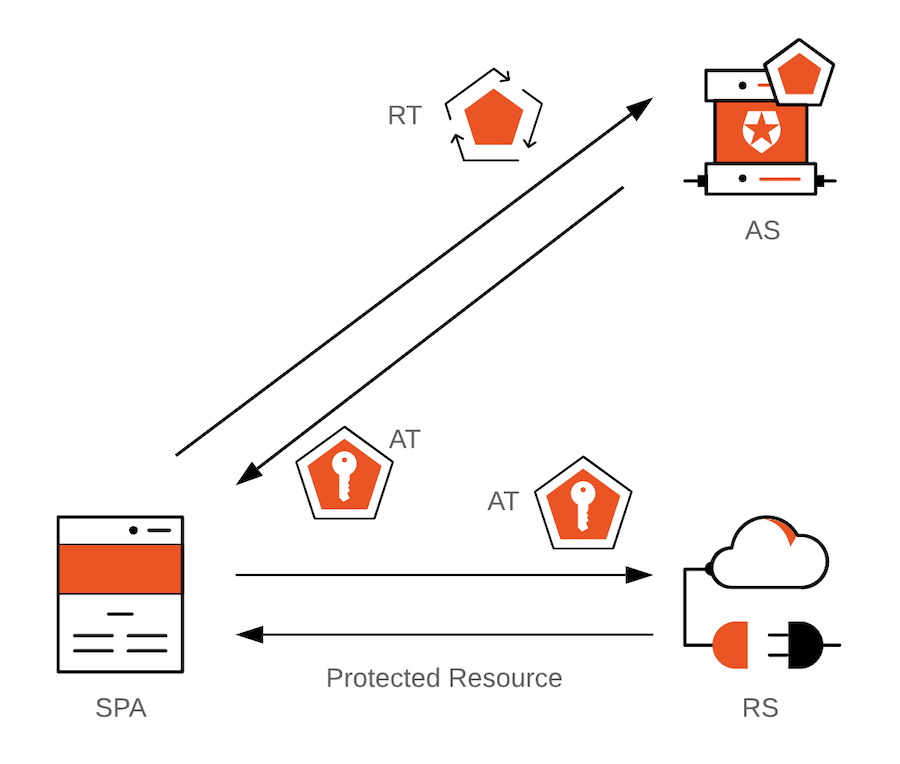
\includegraphics[width=0.7\columnwidth]{autenticazione/rt-and-at} 
    \caption{Flusso dei token JWT. RT = Refresh Token; AT = Access Token; AS = Authorization Server (Server di Autorizzazione); RS = Resourse Server (Server di Risorsa); SPA = Single Page Application (Applicazione Web). Fonte: \cite{site:jwt-flow}}
	\label{fig:jwt-flow}
\end{figure}

\section{Standard di sicurezza per JWT}
I \emph{JWT} sono uno standard aperto e flessibile, il che significa che possono essere utilizzati in molti contesti diversi.
Tuttavia, per garantire la sicurezza dei token e dei dati che contengono, è importante seguire alcune \emph{best practices}\footnote{Le best practices (migliori pratiche) sono linee guida raccomandate per ottenere risultati ottimali. Seguendo queste linee guida, si possono evitare errori comuni e migliorare efficienza, qualità e sicurezza di processi e prodotti.} e standard di sicurezza.

\subsection{JSON Web Encryption}
Il \emph{\gls{JWE}} standard stabilisce un modo per crittografare, e quindi rendere oscuri, i contenuti di un \emph{JWT}.
A primo impatto, potrebbe sembrare che la crittografia abbia le stesse garanzie della firma, con l'aggiunta della riservatezza dei dati.
Tuttavia la crittografia non garantisce l'autenticità dei dati, ma solo la loro riservatezza.

Il \emph{JWE} supporta principalmente due schemi: uno schema a chiave segreta e uno a chiave pubblica.
Lo schema a chiave segreta funziona in modo che ogni parte che detiene la chiave segreta può crittografare e decrittografare i dati

Lo schema a chiave pubblica, invece, funziona in maniera differente.
In questo caso sono le parti che detengono la chiave pubblica a crittografare i dati, mentre la parte che detiene la chiave privata può decrittografarli.
In pratica, chi detiene la chiave pubblica può creare nuovi messaggi crittografati.
Questo, però, non vuol dire che chi crittografa i dati è sempre chi sostiene di essere. Di conseguenza, la crittografia non può fornire le stesse garanzie di autenticità come per la firma.

Per questi motivi \emph{JWE} è spesso utilizzato in combinazione con \emph{\gls{JWS}}: un token crittografato funziona da container per un token firmato in modo da ottere i benefici di entrambi.

\subsection{JSON Web Signature}
Il \emph{JSON Web Signature (JWS)} stabilisce un singolo algoritmo di firma supportato da tutte le implementazioni: \emph{\hyperref[sec:hmac]{HMAC}} con \emph{\gls{SHA-256}}, chiamato \emph{HS256}.
Tuttavia, secondo il \emph{\gls{JWA}} standard, anche altri algoritmi sono consigliati per l'uso con \emph{JWT}.
Tra questi \emph{\hyperref[sec:rsassa]{RSASSA PKCS1 v1.5}} con \emph{SHA-256 (RS256)} e \emph{\hyperref[sec:ecdsa]{ECDSA}} con \emph{\gls{P-256}} a curva ellittica e \emph{SHA-256 (ES256)}\footnote{Questi algoritmi vengono descritti nei paragrafi successivi}.


\section{HMAC}
\label{sec:hmac}

\emph{Keyed-Hash Message Authentication Code (HMAC)} è un algoritmo di firma che combina un certo messaggio con una chiave segreta utilizzando una funzione \emph{hash} crittografica.
Il risultato è un codice di autenticazione che può essere utilizzato per verificare un messaggio solo se le parti generatrice e verificatrice condividono la stessa chiave segreta.

La robustezza della funzione \emph{hash} garantisce che il messaggio non possa essere modificato senza conoscere la chiave segreta.

In sostanza, \emph{HMAC} permette di verificare l'integrità e l'autenticità di un messaggio attraverso chiavi segrete condivise.

\noindent Sia:
\begin{itemize}
	\item $H$ la funzione \emph{hash} crittografica
	\item $B$ la lunghezza del blocco di $H$
	\item $K$ la chiave segreta
	\item $K'$ la vera chiave utilizzata da $H$ e derivata da $K$
	\item $ipad$ il byte \emph{0x36} ripetuto $B$ volte (chiamato anche padding interno)
	\item $opad$ il byte \emph{0x5C} ripetuto $B$ volte (chiamato anche padding esterno)
	\item $M$ il messaggio
	\item $||$ l'operatore di concatenazione
\end{itemize}

\noindent L'algoritmo \emph{HMAC} è definito come:
% \begin{verbatim}
\begin{equation}
	\begin{aligned}
		&HMAC(K, M) = H((K' \oplus opad) || H((K' \oplus ipad) || M))
	\end{aligned}
\end{equation}

\noindent dove $\oplus$ è l'operatore di \emph{XOR}\footnote{Lo XOR (o OR esclusivo) è un'operazione binaria che restituisce 1 se e solo se uno degli operandi è 1, altrimenti restituisce 0} e $K'$ è definito come segue:
\begin{itemize}
	\item Se $K$ è più corto di $B$, vengono aggiunti zeri a sinistra per raggiungere la lunghezza di $B$.
	\item Se $K$ è più lungo di $B$, viene calcolato $H(K)$.
	\item Se $K$ è esattamente di $B$ byte, $K'$ è uguale a $K$.
\end{itemize}

\noindent La funzione \emph{HS256} è un esempio di algoritmo \emph{HMAC} che utilizza la funzione di \emph{hash} \emph{SHA-256}.


\section{RSA}
Gli algoritmi a chiave pubblica si basano sulla generazione di due chiavi, una privata e una pubblica, per crittografare e decrittografare rispettivamente i dati.

L'algoritmo \emph{RSA}, uno dei più noti algoritmi a chiave pubblica, si fonda sulla complessità del problema della fattorizzazione dei numeri interi composti.
La sicurezza di \emph{RSA} deriva dal fatto che, mentre è relativamente facile moltiplicare due numeri primi per ottenere un numero composto, è estremamente difficile eseguire l'operazione inversa, ossia fattorizzare un numero composto per ottenere i due numeri primi originali.

\noindent Questo problema può essere rappresentato come segue:
\begin{equation}
	\begin{aligned}
		&(m^e)^d \equiv m \mod n
	\end{aligned}
\end{equation}

\noindent $m$ è il messaggio originale ed $e$, $d$ e $n$ sono scelti nel seguente modo:
\begin{enumerate}
	\item $p$ e $q$ sono due grandi primi generati casualmente.
	      \begin{itemize}
		      \item Un \emph{\gls{RNG}} crittograficamente sicuro dovrebbe essere utilizzato per generare questi numeri.
		      \item Non esistendo modo di generare randomicamente numeri primi, è necessario verificare che i numeri generati siano effettivamente primi.
		      \item I numeri primi devono essere grandi e simili per ordine di grandezza.
	      \end{itemize}
	\item $n$ è il risultato del prodotto $p \cdot q$. Questo numero è il modulo e il suo numero di bit equivale alla lunghezza della chiave.
	\item $\phi(n) = (p - 1) \cdot (q - 1)$ è il quoziente di Eulero ($phi(n)$).
	\item $e$ è un numero intero scelto in modo che $1 < e < \phi(n)$ e $e$ sia coprimo con $\phi(n)$.
	\item $d$ deve soddisfare la congruenza $d \equiv e^{-1} \mod \phi(n)$.
	      \begin{itemize}
		      \item $d$ è l'inverso moltiplicativo di $e$ modulo $\phi(n)$.
		      \item L'equazione può essere riscritta come $e \cdot d \equiv 1 \mod \phi(n)$.
	      \end{itemize}
\end{enumerate}

La chiave pubblica è composta dai valori di $n$ ed $e$, mentre la chiave privata è composta dai valori di $n$ e $d$.

$p$, $q$ e $\phi(n)$ sono valori che devono essere mantenuti segreti.

Questa proprietà consente a chiunque abbia la chiave pubblica di crittografare un messaggio, ma solo chi possiede la chiave privata sarà in grado di decrittografarlo.

\subsection{Firma e Verifica con RSA}
\label{sec:rsassa}

L'algoritmo \emph{RSA} non è solo utilizzato per la crittografia, ma anche per la firma digitale.
La caratteristica principale dell'avere una coppia di chiavi pubblica e privata permette di utilizzare \emph{RSA} per creare firme digitali che permettono a chiunque di verificare l'origine e l'integrità del messaggio firmato utilizzando la chiave pubblica.
Infatti, solamente chi è in possesso della chiave privata può creare la firma.
Le chiavi pubbliche invece possono essere distribuite liberamente poichè non permettono di creare nuove firme, ma solo di validarle.

\noindent Il processo di firma e verifica funziona come segue:
\begin{enumerate}
	\item Un \emph{digest}\footnote{Un \emph{digest} è un breve valore risultato da un blocco di dati più grande tramite una funzione \emph{hash}. Funziona come una "impronta digitale" dei dati, permettendo di verificare l'integrità e l'autenticità dei dati stessi senza bisogno di conoscere l'intero contenuto originale.} del messaggio viene calcolato da una funzione hash.
	\item Il \emph{digest} viene poi elevato alla potenza di $d$ modulo $n$ (chiave privata).
	\item Il risultato è aggiunto al messaggio come firma.
\end{enumerate}
\noindent Per verificare la firma invece:
\begin{enumerate}
	\item La firma viene elevata alla potenza di $e$ modulo $n$ (chiave pubblica). Questo restituisce il \emph{digest} originale.
	\item Viene calcolato il \emph{digest} del messaggio ricevuto, utilizzando la stessa funzione \emph{hash} del passaggio di firma.
	\item Se i due \emph{digest} sono uguali, la firma è valida.
\end{enumerate}

Questo processo è conosciuto come \emph{\gls{SSA}}, infatti la firma è un "appendice" del messaggio originale in quanto è necessario nel processo di verifica della firma.
Questo schema permette dunque la possibilità di distribuire in modo sicuro uno-a-molti messaggi firmati: le parti riceventi possono verificare l'autenticità del messaggio mantenendo una copia della chiave pubblica, ma non possono creare nuovi messaggi con essa.

\emph{RSASSA} è una famiglia di schemi di firme digitali basati su \emph{RSA} che utilizzano \emph{SSA}.
Tra questi algoritmi possiamo trovare \emph{RSASSA-PKCS1-v1\_5} che utilizza un tipo di padding specifico descritto nello standard \emph{\gls{PKCS1} v1.5}.
L'utilizzo della funzione di \emph{hash SHA-256} permette di rendere la firma di \emph{RS256}\footnote{RSASSA-PKCS1-v1\_5 con SHA-256} crittograficamente sicura.

\section{ECC}
L'esistenza di algoritmi di fattorizzazione efficienti come il \emph{\gls{GNFS}} o il \emph{\gls{QS}} ha reso \emph{RSA} con chiavi brevi vulnerabile.
Questo ha portato alla necessità di utilizzare chiavi sempre più lunghe per garantire un livello di sicurezza accettabile.
Tuttavia, con l'aumentare della lunghezza delle chiavi, anche il tempo di calcolo per le operazioni \emph{RSA} aumenta significativamente.
Questo compromesso tra sicurezza e performance diventa insostenibile sul lungo periodo, in particolare per dispositivi con risorse limitate.
Ciò può potenzialmente rendere \emph{RSA} insicuro e non più utilizzabile.

L'\emph{ECC} consente di creare algoritmi crittografici più efficienti.
Tra questi, l'\emph{\hyperref[sec:ecdh]{Elliptic Curve Diffie-Hellman (ECDH)}} per lo scambio di chiavi e l'\emph{Elliptic Curve Digital Signature Algorithm (ECDSA)} per la firma digitale sono i più comuni.
Anche questo tipo di algoritmi genera una coppia di chiavi privata/pubblica, ma utilizza, invece della fattorizzazione di numeri semiprimi, il logaritmo discreto su curve ellittiche.

\noindent Le curve ellittiche per la crittografia sono definite dalla seguente equazione di terzo grado:

\begin{equation}
	\begin{aligned}
		&y^2 = x^3 + ax + b
	\end{aligned}
\end{equation}

\noindent dove $a$ e $b$ sono parametri della curva.

Gli algoritmi a curve ellittiche sono definiti su campi primi finiti, ovvero insiemi di numeri interi su cui sono definite due operazioni binarie: somma e moltiplicazione.
Con campo primo finito si intende che il numero di elementi nel campo è un numero primo $p$, quindi una quantità finita. Tutti gli elementi e le operazioni sono definite modulo $p$.

Rendendo il campo finito, gli algoritmi usati per le operazioni matematiche cambiano.
In particolare, il logaritmo discreto viene usato al posto del logaritmo normale.

Essendo il campo composto da un numero finito di elementi, si potrebbe pensare che il logaritmo discreto diventi un problema semplice, tuttavia, non esiste ad oggi un algoritmo efficiente per la risoluzione del logaritmo discreto su curve ellittiche.
Questa proprietà rende il logaritmo discreto ideale per la crittografia e la firma digitale.

Per rendere però l'algoritmo sicuro, è necessario che la curva, ovvero i parametri $a$ e $b$, sia scelta in modo corretto. In passato, infatti, si sono verificati casi in cui certi parametri hanno reso le curve deboli.

\noindent Un esempio di curva ellittica è illustrato in figura \ref{fig:curva-ellittica}. L'equazione della curva è la seguente:

\begin{equation}
	\begin{aligned}
		&y^2 = x^3 - 3x + 25
	\end{aligned}
\end{equation}


\begin{figure}[!ht] 
    \centering 
    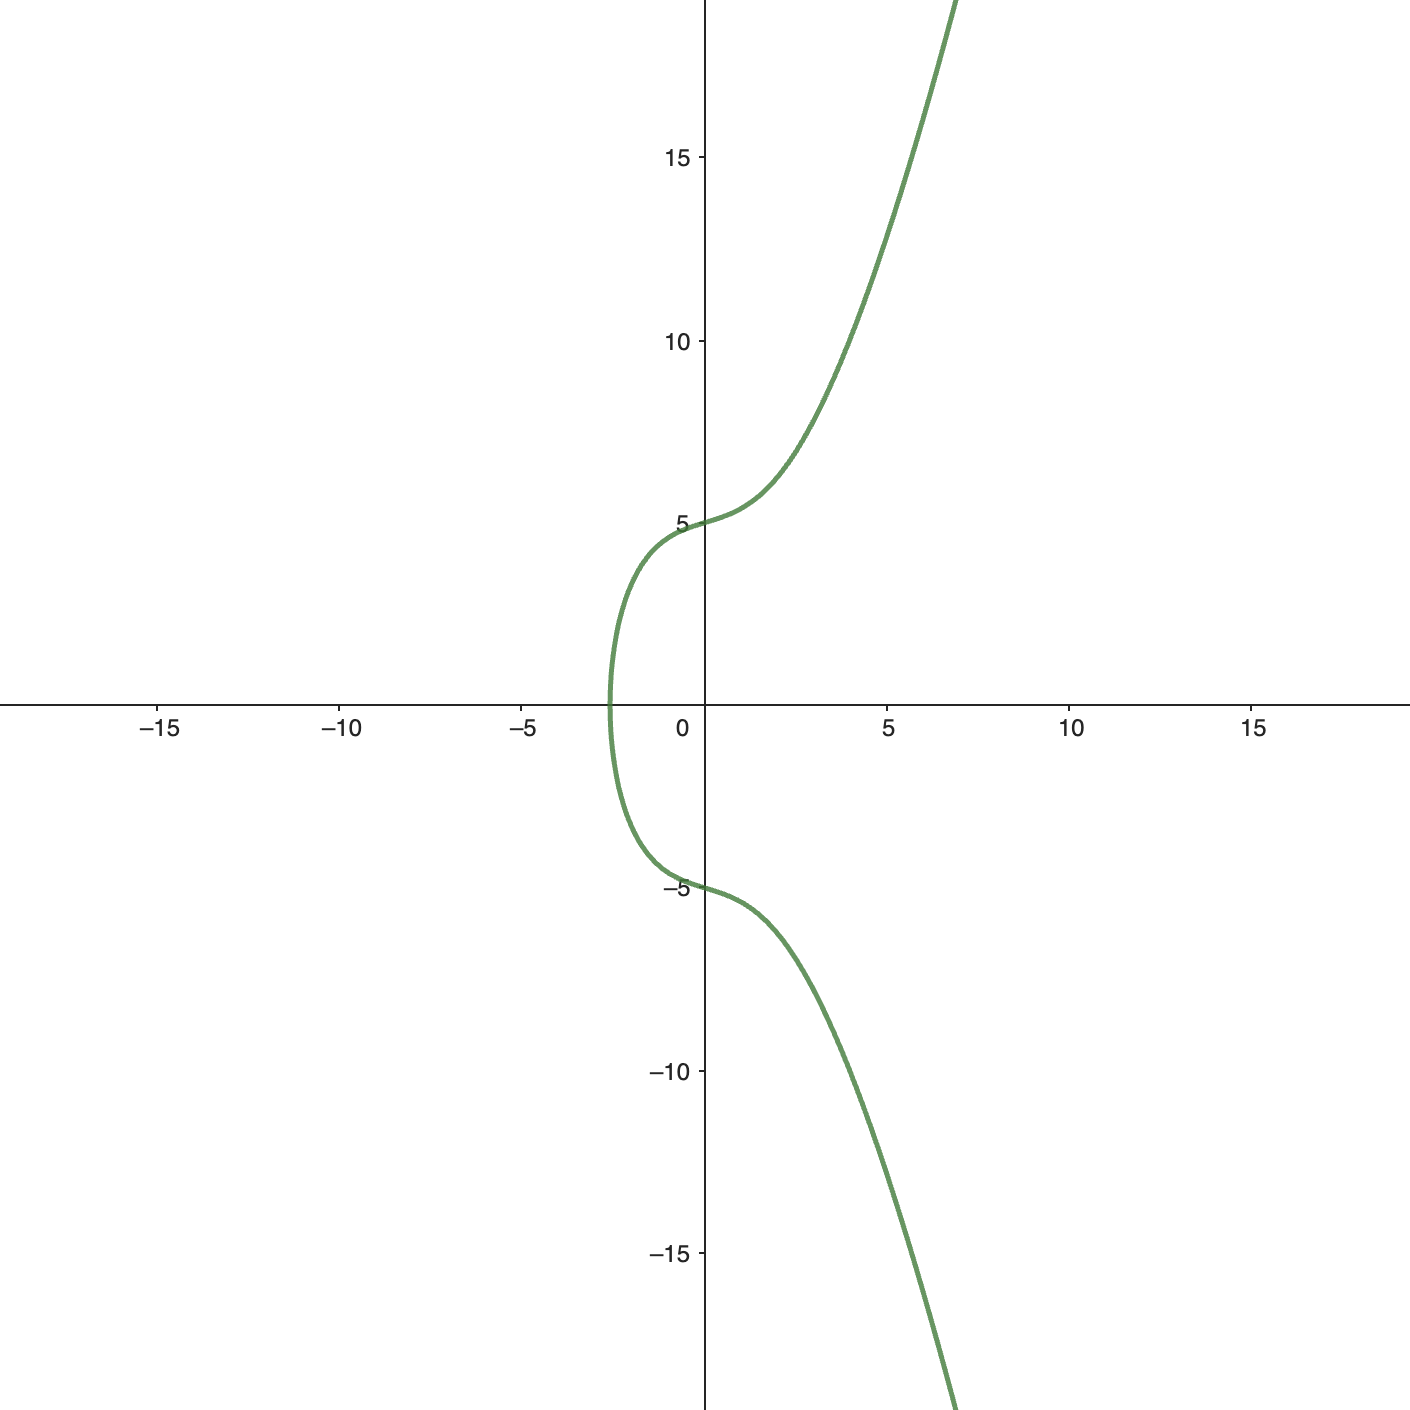
\includegraphics[width=0.7\columnwidth]{autenticazione/curva-ellittica} 
    \caption{Grafico di una curva ellittica}
	\label{fig:curva-ellittica}
\end{figure}

L'aspetto interessante degli algoritmi a curva ellittica è che la lunghezza della chiave può essere ridotta di molto rispetto a \emph{RSA} per ottenere lo stesso livello di sicurezza.
Per esempio, una chiave EC\footnote{Chiave generata da una curva ellittica} di 256 bit è considerata sicura quanto una chiave \emph{RSA} di 3072 bit.

Ciò, oltre che a rendere più efficienti gli algoritmi, semplifica la trasmissione e la memorizzazione delle chiavi.
Il motivo per cui la chiave EC può essere più corta risiede nell'inesistenza, ad oggi, di algoritmi che risolvono il logaritmo discreto più efficientemente dell'approccio \emph{naive} o \emph{brute-force}\footnote{Con \emph{naive} o \emph{brute-force} si intende il "provare" tutti i valori possibili}, diversamente da \emph{RSA} che è più vulnerabile a fattorizzazione efficiente.

In un suo studio, il matematico Arjen K. Lenstra ha esposto il concetto di "Universal Security"\footcite{site:universal-security} calcolando l'energia necessaria per rompere determinti algoritmi crittografici e comparandola con la quantità di acqua che quell'energia sarebbe in grado di portare a ebollizione.
Con questo metodo, Lenstra ha dimostrato che per rompere una chiave \emph{RSA} di 228 bit è richiesta meno energia di quella necessaria per portare a ebollizione un cucchiaino d'acqua.
Al contrario, per rompere una chiave EC a 228 bit è necessaria una quantità di energia che porterebbe a ebollizione l'intera acqua presente sulla Terra.
Per questo livello di sicurezza con \emph{RSA} è necessaria una chiave di almeno 2380 bit.

\subsection{Usi di ECC}
Nonostante la sua sicurezza e la sua efficienza, l'uso di \emph{ECC} è ancora limitato rispetto a \emph{RSA}.
Tuttavia, negli ultimi anni si è assistito ad un aumento nell'interesse per questa tecnologia e ad un incremento del suo utilizzo in varie applicazioni.
Il governo degli Stati Uniti, ad esempio, ha adottato \emph{ECC} per la crittografia delle comunicazioni, il progetto Tor lo utilizza per aiutare a garantire l'anonimato degli utenti e il protocollo \emph{\gls{TLS}} lo utilizza per garantire la sicurezza delle comunicazioni su Internet tramite \emph{\gls{HTTPS}}.
Anche i servizi di messaggistica di iMessage e Whatsapp utilizzano \emph{ECC} per garantire la sicurezza delle loro comunicazioni.
\emph{ECC} è inoltre utilizzato in molte applicazioni di blockchain, come Bitcoin ed Ethereum, al fine di approvare le transazioni.

\subsection{Elliptic Curve Digital Signature Algorithm (ECDSA)}
\label{sec:ecdsa}

L'\emph{Elliptic Curve Digital Signature Algorithm} è un algoritmo di firma digitale basato su curve ellittiche.
Il funzionamento è simile a quello di \emph{RSA}, ma utilizza curve ellittiche al posto dei numeri interi.

Immaginiamo che \emph{Utente A} voglia inviare un messaggio firmato a \emph{Utente B}.
\emph{A} sceglie in modo randomico un numero $d_A$ nel range $[1, n-1]$, che rappresenta la chiave private e dove $n$ è l'ordine del punto base $G$ della curva ellittica ed è un numero primo.
A questo punto, \emph{A} calcola il punto $Q_A = d_A \cdot G$\footnote{Nel contesto delle curve ellittiche indicheremo con il $\cdot$ del prodotto scalare la "moltiplicazione scalare delle curve ellittiche" (dall'inglese elliptic curve point multiplication). Questa è un'operazione che consiste nel sommare ripetutamente un punto $P$ sulla curva a se stesso un certo numero di volte $k$. La nomenclatura risulterà $P \cdot k$. \cite{site:ec-point-multiplication}} e la coordinata $x$ di $Q_A$. Il risultato è un punto della curva che rappresenta la chiave pubblica.
La curva ellittica e i suoi parametri (inclusi $G$ e $n$) vengono prestabiliti in base a uno standard crittografico.

\noindent Dunque, per firmare un messaggo \emph{Utente A} procede come segue:
\begin{enumerate}
	\item Calcola il digest $H(m)$ del messaggio $m$ con una funzione hash crittografica.
	\item $H(m)$ viene poi convertito in un numero intero intero $h$ ridotto modulo $n$.
	\item Un numero $k$ viene scelto randomicamente nel range $[1, n-1]$.
	\item Calcola il punto $k \cdot G$ e la sua coordinata $x$ viene ridotta modulo $n$, ottenendo $r$. Se $r = 0$, viene scelto un nuovo $k$.
	\item Calcola $s = (h + r \cdot d_A)/k \mod n$. Se $s = 0$, viene scelto un nuovo $k$.
	\item La coppia $(r, s)$ è la firma del messaggio.
\end{enumerate}

\noindent È importante notare che $k$ deve essere scelto in modo randomico e non deve essere mai riutilizzato con la stessa chiave privata.
L'utilizzo di $k$ più volte con la stessa chiave privata può portare alla compromissione della chiave privata.

\noindent Per verificare la firma \emph{Utente B} procede come segue:
\begin{enumerate}
	\item Verifica che $r$ e $s$ siano nel range $[1, n-1]$ e che $Q_A$ sia un punto sulla curva il cui prodotto con $n$ è l'elemento neutro.
	\item Calcola il digest $H(m)$ del messaggio $m$ con una funzione hash crittografica.
	\item $H(m)$ viene poi convertito in un numero intero intero $h$ ridotto modulo $n$.
	\item Calcola $w = s^{-1} \mod n$.
	\item Calcola $u_1 = hw \mod n$ e $u_2 = rw \mod n$.
	\item Calcola il punto $u_1 \cdot G + u_2 \cdot Q_A$ e la sua coordinata $x$ viene ridotta modulo $n$, ottenendo $v$.
	\item La firma è valida se $v = r$.
\end{enumerate}

\noindent \emph{ES256} è un esempio di algoritmo \emph{ECDSA} che utilizza la funzione di \emph{hash} \emph{SHA-256}.


\section{Diffie Hellman Key Exchange}
Il \emph{Diffie-Hellman Key Exchange (D-H)} è un protocollo crittografico che permette a due parti che non hanno una conoscenza pregressa di stabilire una chiave segreta condivisa su un canale di comunicazione non sicuro.
Questo protocollo fornisce le basi per una varietà di diversi protocolli crittografici. In particolare, è alla base della perfetta segretezza di \emph{TLS}, il protocollo utilizzato da \emph{HTTP(S)} per garantire la sicurezza delle comunicazioni.
Il protocollo originale, sviluppato da Whitfield Diffie e Martin Hellman nel 1976, non prevedeva la firma digitale e quindi non garantiva l'autenticità delle parti coinvolte nella comunicazione, rendendo il protocollo vulnerabile al \emph{\gls{MITM}}.

L'algoritmo si basa sulla difficoltà di calcolare il logaritmo discreto su campi finiti.
Inizialmente, le due parti scelgono un numero primo $p$ e un generatore $g$ del campo finito tale che $g^x \mod p$, per $x = 1, 2, ..., p-1$, generi tutti gli elementi del campo in qualche permutazione.
Per ogni intero $b$ minore di $p$ e radice primitiva di $p$, esiste un unico esponente $i$ tale che $b = a^i \mod p$. Questo esponente è chiamato logaritmo discreto di $b$ in base $a$ modulo $p$.

Supponiamo che \emph{Utente A} e \emph{Utente B} vogliano stabilire una chiave segreta condivisa. Il protocollo funziona come segue:
un numero primo $p$ e un intero $\alpha$, che è una radice primitiva di $p$, vengono scelti e resi pubblici. Gli utenti \emph{A} e \emph{B} scelgono in modo casuale rispettivamente due numeri segreti $X_a$ e $X_b$ minori di $p$ e calcolano $Y_a = \alpha^{X_a} \mod p$ e $Y_b = \alpha^{X_b} \mod p$.
Dopodiché, \emph{A} e \emph{B} scambiano i loro valori pubblici $Y_a$ e $Y_b$ mantenendo segreti i loro valori privati $X_a$ e $X_b$.
Infine, \emph{A} calcola $K = Y_b^{X_a} \mod p$ e \emph{B} calcola $K = Y_a^{X_b} \mod p$. Entrambi otterranno lo stesso valore $K$ che sarà la chiave segreta condivisa.
Infatti:

\begin{equation}
	\begin{aligned}
		&K = Y_b^{X_a} \mod p \\
		&= (\alpha^{X_b} \mod p)^{X_a} \mod p \\
		&= \alpha^{X_a \cdot X_b} \mod p \\
		&= \alpha^{X_b \cdot X_a} \mod p \\
		&= (\alpha^{X_a} \mod p)^{X_b} \mod p \\
		&= Y_a^{X_b} \mod p = K
	\end{aligned}
\end{equation}

In questo modo i due utenti si sono scambiati una chiave segreta senza che nessuno dei due abbia mai inviato la propria chiave privata.
Inoltre, un attaccante che intercetta i valori pubblici $Y_a$ e $Y_b$ non può risalire ai valori privati $X_a$ e $X_b$ senza conoscere il logaritmo discreto su campi finiti.
La sicurezza del protocollo si basa sulla relativa facilità di calcolare esponenziali modulari e la difficoltà di calcolare logaritmi discreti. In particolare, per primi grandi, quest'ultima operazione è considerata infattibile.


\subsection{Autenticazione in Diffie Hellman}
Nonostante l'efficacia dello scambiare chiavi segrete, il protocollo \emph{Diffie-Hellman (D-H)} originale non prevedeva l'autenticazione delle parti coinvolte nella comunicazione, rendendolo vulnerabile a MITM e \emph{\gls{Impersonation Attack}}.

Nell'\emph{Impersonation Attack}, l'attaccante intercetta un messaggio di \emph{A} indirizzato a \emph{B}, contenente la chiave pubblica $Y_a$, e invia ad \emph{A} la propria chiave pubblica $Y_{att}$ con l'\emph{User ID} di \emph{B}.
In questo modo \emph{A} genera la chiave segreta condivisa credendo di star comunicando con \emph{B}.

Nel \emph{Man-in-the-Middle Attack}, un attaccante si interpone tra le due parti e stabilisce due connessioni separate, una con \emph{A} e una con \emph{B}, impersonando entrambe le parti. Il \emph{MITM} può essere effettuato anche tra un utente e un server. Questo processo viene illustrato in figura \ref{fig:mitm}.

\begin{figure}[!ht] 
    \centering 
    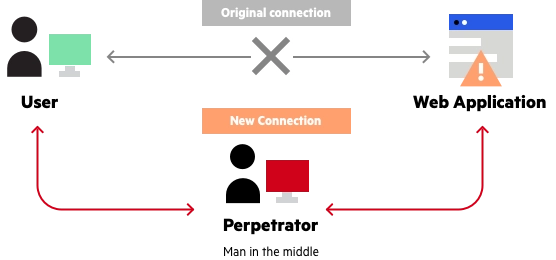
\includegraphics[width=0.8\columnwidth]{autenticazione/mitm} 
    \caption{Man in the Middle Attack \cite{site:mitm-image}}
	\label{fig:mitm}
\end{figure}

Si può notare come il protocollo è soggetto a questo tipo di attacchi in quanto non è presente nessun tipo di autenticazione tra le parti.

\noindent Esistono generalmente tre metodi differenti per garantire l'autenticità delle parti in \emph{D-H}:
\begin{itemize}
	\item \textbf{Firma Digitale}: Lo scambio di chiavi è autenticato da una firma, ovvero un \emph{hash} ottenibile da entrambi gli utenti, ciascuno crittografato con la propria chiave privata. Questo \emph{hash} viene generato da parametri importanti come l'\emph{User ID}.
	\item \textbf{Cifratura a chiave pubblica}: Alcuni parametri importanti vengono crittografati con la propria chiave privata.
	\item \textbf{Chiave simmetrica}: Una chiave simmetrica condivisa attraverso altri mezzi viene utilizzata per autenticare la comunicazione.
\end{itemize}

\subsection{Diffie Hellman Key Exchange con Curve Ellittiche}
\label{sec:ecdh}

Il \emph{Diffie-Hellman Key Exchange} può essere implementato anche con curve ellittiche. Questo protocollo, chiamato \emph{Elliptic Curve Diffie-Hellman (ECDH)}, funziona in modo simile al \emph{D-H} tradizionale, ma utilizza curve ellittiche al posto dei numeri interi.
\emph{Utente A} and \emph{B} scelgono una curva ellittica $E(a,b)$ e un punto $G$ su di essa, che funge da generatore. Questi parametri vengono resi pubblici.
\emph{A} e \emph{B} scelgono, a questo punto, due numeri casuali e segreti $X_a$ e $X_b$ e calcolano rispettivamente $Y_a = X_a \cdot G$ e $Y_b = X_b \cdot G$, dove $\cdot$ indica il prodotto scalare.
\emph{A} e \emph{B} si scambiano i valori pubblici $Y_a$ e $Y_b$ e calcolano grazie ad essi la chiave segreta condivisa $K$.
\begin{equation}
	\begin{aligned}
		&K = X_a \cdot Y_b\\
		&= X_a \cdot (X_b \cdot G)\\
		&= X_b \cdot (X_a \cdot G)\\
		&= X_b \cdot Y_a = K
	\end{aligned}
\end{equation}

Anche in questo caso, un utente malevolo che intercetta i valori pubblici $Y_a$ e $Y_b$ non può risalire ai valori privati $X_a$ e $X_b$ senza conoscere il logaritmo discreto su curve ellittiche e quindi non può ottenere la chiave segreta condivisa.

Come per il \emph{D-H} tradizionale con numeri interi, anche \emph{ECDH} non prevede l'autenticazione delle parti coinvolte nella comunicazione e quindi è vulnerabile a \emph{MITM Attack}.


\section{Considerazioni sulla Sicurezza di JWT}
Come già detto, La firma digitale garantisce l'integrità dei dati contenuti nei token JWT, ma per assicurare una completa sicurezza è fondamentale considerare alcuni aspetti cruciali.
Innanzitutto, è necessario archiviare correttamente le chiavi, garantendo che siano al sicuro e non siano accessibili a terzi.
Ciò è ugualmente importante nel caso di token crittografati.

Un altro aspetto importante è la trasmissione di informazioni sensibili.
Per evitare la divulgazione di questi dati durante la trasmissione dei token è estremamente consigliato utilizzare protocolli sicuri come \emph{HTTPS}.
Inoltre, la cifratura dei token rappresenta un ulteriore livello di protezione, particolarmente utile quando i token contengono dati sensibili.

Nel caso in cui siano necessarie sia la firma che la crittografia, è consigliabile firmare il token prima di crittografarlo.
Questo approccio previene attacchi come il \emph{Signature Stripping Attack}, in cui l'attaccante tenta di rimuovere la firma dal token per ottenere accesso ai dati.

Oltre a ciò, è essenziale implementare una corretta gestione dei token. Questo include la limitazione della durata dei token tramite scadenze brevi e l'adozione di un sistema di revoca per invalidare i token compromessi o non più validi. È anche importante applicare politiche di rotazione delle chiavi, limitando il periodo di validità delle chiavi e sostituendole regolarmente.

\subsection{Signature Stripping Attack}
Un metodo comune per aggirare la verifica della firma consiste nel rimuovere la firma dal token.
Essendo le tre parti del token codificate separatamente, un attaccante può facilmente rimuovere la firma e modificare l'\emph{header} per far sembrare il token valido senza una firma.

Per prevenire efficacemente questo attacco è essenziale assicurarsi che il server accetti solo token firmati. Questo controllo deve essere rigoroso per garantire che solo token autentici vengano utilizzati all'interno del sistema.

\subsection{Cross-Site Request Forgery Attack}
Attacchi \emph{Cross-Site Request Forgery Attack (CSRF)} sfruttano la fiducia che un sito ha in un utente autenticato per inviare richieste non autorizzate, ingannando il browser dell'utente a inviare richieste a un sito diverso da quello visitato attraverso elementi come immagini o script che contengono l'\emph{URL} del sito target.
Se il sito target utilizza cookie di sessione, queste richieste conterranno automaticamente le credenziali dell'utente.

\emph{JWT} token con breve validità di tempo possono mitigare questo attacco, in modo da poter ridurre il tempo in cui un token rubato può essere sfruttato.
Un'altra soluzione efficace è l'use di speciali campi che vengono aggiunti alle richieste solo quando provengono da un sito autorizzato.
Inoltre, poiché l'attacco CSRF si basa sui cookie, evitare di memorizzare i token JWT nei cookie può prevenire l'attacco, utilizzando invece altre tecniche di memorizzazione.

\subsection{Cross-Site Scripting Attack}
Gli attacchi \emph{Cross-Site Scripting Attack (XSS)} consentono a un attaccante di eseguire script malevoli nel browser di un utente.
Questi script possono essere utilizzati per rubare i token accedendo ai cookie e al \emph{localStorage}.

Molti attacchi \emph{XSS} sono causati da una mancata validazione e sanificazione dei dati passati al server.
Infatti, se il \emph{backend}\footnote{Il \emph{backend} è la parte di un'applicazione che si occupa dell'elaborazione dei dati e della logica dell'applicazione.} non sanifica i dati in ingresso, un attaccante può inserire dati in modo che vengano interpretati come script.

Per risolvere questo problema è sempre necessario sanificare i dati in ingresso.
Inoltre, se i token vengono salvati nei cookie, è possibile utilizzare la flag \emph{HttpOnly} per impedirne l'accesso da parte di script eseguiti nel browser.
